% \newpage
\subsection{Fancier optimization}
SGD
\begin{align*}
    x_{t+1}=x_t-\alpha\nabla f(x_t)
\end{align*}
\begin{lstlisting}[language={python}]
while True:
    dx=compute_gradient(x)
    x+=learning_rate*dx
\end{lstlisting}

\subsubsection{Probelms with SGD}
\begin{enumerate}
    \item 若loss在不同方向上的敏感度相差较大, 则SGD所给出的梯度可能不会准确指向目标. 如 \textbf{Figure} \ref{SGDP1}. 即loss function二阶偏导Hessian矩阵拥有更高的\textbf{条件数}: 向量在经过Hessian矩阵变换后其长度的最大放大倍数与最小放大倍数之比更大. 

    \begin{figure}[!htb]
        \centering
        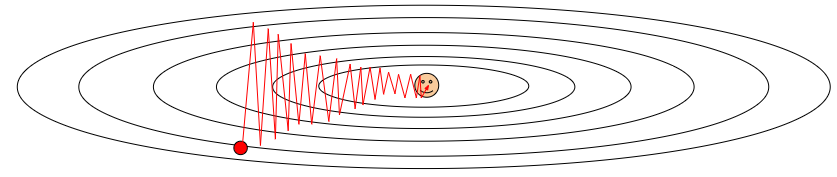
\includegraphics[width=0.42\textwidth]{pic/Lec7/SGDP1.png}
        \caption{loss 在水平方向变换小, 在垂直方向变化大. }
        \label{SGDP1}
    \end{figure}
    \item local minima (局部最小值) or saddle point (鞍点), 他们的梯度为0, 会困住 SGD. 在更高维的空间之中, 鞍点更加常见. 在鞍点附近的梯度会很小, 让SGD前进缓慢. 
    \begin{figure}[!htb]
        \centering
        \begin{minipage}{0.22\textwidth}
            \centering
            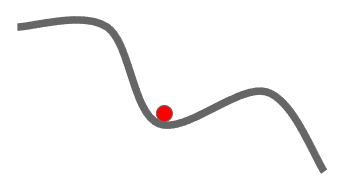
\includegraphics[height=0.5\textwidth]{pic/Lec7/local minima.png}
            \caption{local minima}
        \end{minipage}
        \begin{minipage}{0.22\textwidth}
            \centering
            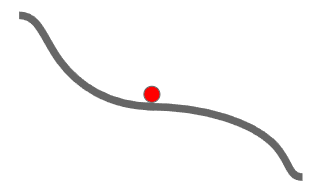
\includegraphics[height=0.5\textwidth]{pic/Lec7/saddle point.png}
            \caption{saddle point}
        \end{minipage}
    \end{figure}
    \item SGD 是随机的梯度下降. 因为每次迭代计算全部梯度过于昂贵, 所以只随机计算部分的梯度. 但这些梯度可能会来组与噪声, 以导致错误的方向. 
\end{enumerate}

\subsubsection{First-Order Optimization}
\paragraph{SGD + Momentum}
建立``速度''作为梯度的运行平均值, $\rho$ 给予了 ``摩擦力'', 一般 $\rho=0.9 \text{ or } 0.99$. 
\begin{align*}
    v_{t+1}&=\rho v_t+\nabla f(x_t)\\
    x_{t+1}&=x_t-\alpha v_{t+1}
\end{align*}

\begin{lstlisting}[language={python}]
vx=0
while True:
    dx=compute_gradient(x)
    vx=rho*vx+dx
    x+=learning_rate*vx
\end{lstlisting}

此策略有助于解决上面提出的SGD三大问题.

\begin{figure}[!htb]
    \centering
    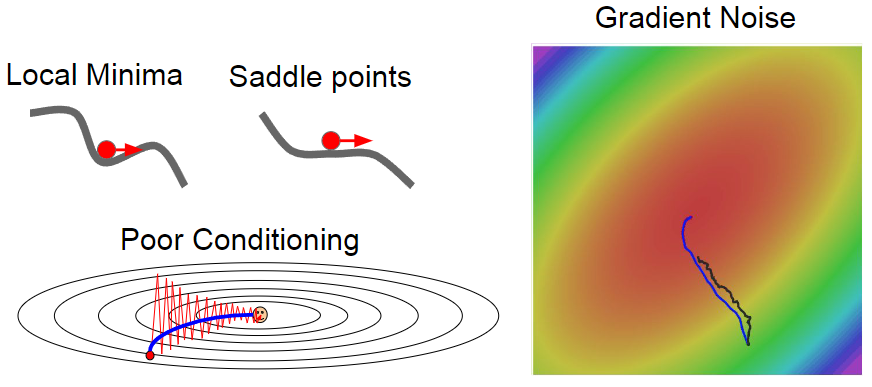
\includegraphics[width=0.42\textwidth]{pic/Lec7/SGDP.png}
    \caption{SGD Probelms}
\end{figure}

\begin{figure}[!htb]
    \centering
    \begin{subfigure}{0.22\textwidth}
        \centering
        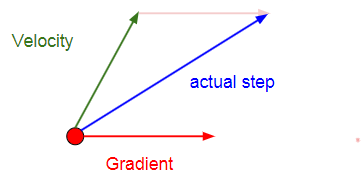
\includegraphics[width=\textwidth]{pic/Lec7/Momentum update}
    \end{subfigure}
    \begin{subfigure}{0.22\textwidth}
        \centering
        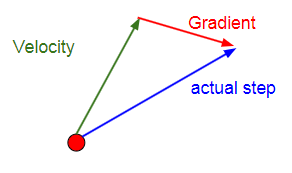
\includegraphics[width=\textwidth]{pic/Lec7/Nesterov Momentum}
    \end{subfigure}
    \caption{Momentum update and Nesterov Momentum}
\end{figure}


\paragraph{Nesterov Momentum} 梯度混合了速度的信息, 有可能纠正错误的速度方向. 
\begin{align*}
    v_{t+1}&=\rho v_t - \alpha \nabla f(x_t+\rho v_t)\\
    x_{t+1}&=x_t+v_{t+1}
\end{align*}
Usually we want update in terms of $x_t$, $\nabla f(x_t)$. So change of variables $\tilde{x}_t=x_t+\rho v_t$ and rearrange:
\begin{align*}
    v_{t+1}&=\rho v_t -\alpha \nabla f(\tilde{x}_t)\\
    \tilde{x}_{t+1}&=\tilde{x}_t-\rho v_t + (1+\rho )v_{t+1}\\
    &=\tilde{x}_t +v_{t+1}+\rho (v_{t+1}-v_t)
\end{align*}
\begin{lstlisting}[language={python}]
v=0
while True:
    dx=compute_gradient(x)
    old_v=v
    v=rho*v-learning_rate*dx
    x+=-rho*old_v+(1+rho)*v
\end{lstlisting}

我们更倾向于更大范围的最小值, 而不某个尖锐的最小值(因为这可能是过拟合). SGD会跳过这些尖锐的最小值, 这是特性, 不是bug [ac01]. 

\paragraph{AdaGrad}添加了基于每个维度的历史平方和的梯度逐元素缩放. 
\begin{lstlisting}[language={python}]
grad_squared=0
while True:
    dx=compute_gradient(x)
    grad_squared+=dx*dx
    x-=learning_rate*dx/(np.sqrt(grad_squared)+1e-7)
\end{lstlisting}

走的长度与梯度大小成一定的反比. 但随着时间增加, 所有的梯度都会变小. 在凸的条件下这很好, 但非凸的话可能会在不应该停的地方停下, 比如鞍点. 

\paragraph{RMSProp} 让grad\_squared以一定参数进行衰减. 
\begin{lstlisting}[language={python}]
grad_squared=0
while True:
    dx=compute_gradient(x)
    grad_squared+=decay_rate*grad_squared+(1-decay_rate)*dx*dx
    x-=learning_rate*dx/(np.sqrt(grad_squared)+1e-7)
\end{lstlisting}

\paragraph{Adam} 有点像有 Momentum + RMSProp 以及一阶矩和二阶矩估计值从0开始的偏差校正. 
\begin{lstlisting}[language={python}]
first_moment=0
second_moment=0
for t in range(num_iterations):
    dx=compute_gradient(x)
    first_moment=beta1*first_moment+(1-beta1)*dx
    second_moment=beta2*second_moment+(1-beta2)*dx*dx
    first_unbias=first_moment/(1-beta1**t)
    second_unbias=second_moment/(1-beta2**t)
    x-=learning_rate*first_unbias/(second_unbias**0.5+1e-7)
\end{lstlisting}
但当第一次迭代时, 如果用0初始化 二阶矩估计, 会让步长非常的大, 且因为 beta2 接近1, 所以会一致持续这种情况. 

\paragraph{Learning rate decay}
让学习率随着时间衰减, 诸如:
\begin{itemize}
    \item exponential decay
    \begin{align*}
        \alpha=\alpha_0 e^{-kt}
    \end{align*}
    \item $1/t$ decay
    \begin{align*}
        \alpha=\frac{\alpha_0}{1+kt}
    \end{align*}
\end{itemize}

设置学习率的衰减最好是观察loss曲线, 看哪里不降了然后尝试在那时衰减学习率, 衰减作为二阶超参数较难优化. 

\paragraph{First-Order Optimization}
\begin{enumerate}
    \item 使用梯度构建线性近似
    \item 迭代使近似最小化
\end{enumerate}

\begin{figure}[!htb]
    \centering
    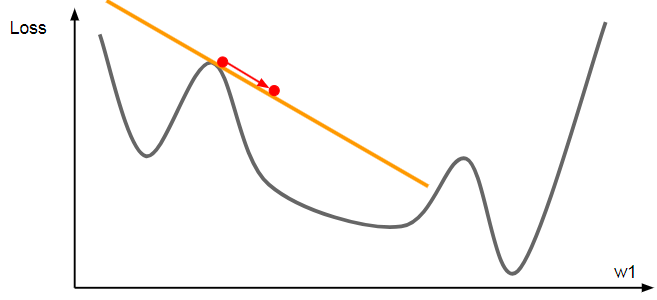
\includegraphics[width=0.309\textwidth]{pic/Lec7/First-Order Optimization}
    \caption{First-Order Optimization}
\end{figure}

\subsubsection{Second-Order Optimization}
\begin{enumerate}
    \item 使用梯度与 Hessian 构建 二次近似
    \item 迭代到近似的最小值
\end{enumerate}

使用牛顿法, second-order Taylor expansion:
\begin{align*}
    J(\mathbf{\theta})\approx J(\mathbf{\theta}_0)+(\mathbf{\theta}-\mathbf{\theta}_0)^T\nabla_{\mathbf{\theta}}J(\mathbf{\theta}_0)+\frac{1}{2}(\mathbf{\theta}-\mathbf{\theta}_0)^T\mathbf{H}(\mathbf{\theta}-\mathbf{\theta}_0)
\end{align*}
Solving for the critical point we obtain the Newton parameter update:
\begin{align*}
    \mathbf{\theta}^*=\mathbf{\theta}_0-\mathbf{H}^{-1}\nabla_{\mathbf{\theta}}J(\mathbf{\theta}_0)
\end{align*}

没有超参数与学习率, 但 Hessian 有 $O(N^2)$ 个元素, 求逆需要 $O(N^3)$, 且一般来说 $N$ 数千万或数亿. 

所以使用些拟牛顿法:
\begin{itemize}
    \item Quasi-Newton methods (e.g. BGFS)
    \item L-BFGS 
    \subitem 通常在整个数据集做 Batch, 确定的模式之下较优
    \subitem 不能很好地转换为小批量设置, 难以处理随机情况. 
\end{itemize}

In practice:
\begin{itemize}
    \item 在大多数情况下, Adam是一种不差的默认设置
    \item 如果有能力把整个数据集作为一个batch做更新, 那可以逝逝 L-BFGS. 
\end{itemize}

\subsection{Model Ensembles}
优秀的优化算法可以利于降低training loss, 但更重要的是降低 train data 与 val data 之间的准确率差距. 

模型集成:
\begin{enumerate}
    \item 独立训练多个模型
    \item 在测试时平均他们的结果
\end{enumerate}

Tips and Tricks:
\begin{enumerate}
    \item 比起独立训练多个模型, 也可以选择在训练过程中保存多次模型的快照. 
    \item 不使用实际的参数向量,而是保持参数向量的移动平均值,并在测试时使用该值(Polyak平均值)
\end{enumerate}

\subsection{Regularization}
\subsubsection{Dropout}
在每次正向传递中, 随机将一些神经元设置为零. 

Dropout 概率是一个超参数; 0.5是常见的. 

\begin{figure}[!htb]
    \centering
    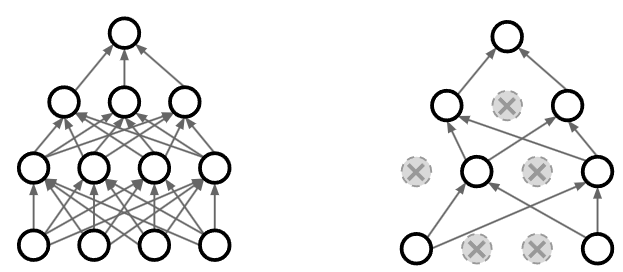
\includegraphics[width=0.42\textwidth]{pic/Lec7/Dropout}
    \caption{Dropout}
\end{figure}

Dropout 强制网络构建有冗余的表示, 放置过于依赖某个特征. 或者说这更类似于模型的集成, dropout 后不同的网络是不同的集成. 

In Test time, 需要剔除输出的随机性, 尝试使用类似的对随机的积分: 
\begin{align*}
    y=f(x)=E_z[f(x,z)]=\int p(z)f(x,z)dz
\end{align*}
$y$为输出, $x$为输入, $z$为决定dropout的随机的mask. 直接积分困难, 尝试近似. 

假设一个简单的神经元 $a=w_1 x+ w_2 y$, dropout概率为0.5. 在 train 时有
\begin{align*}
    E[a]=&\frac{1}{4}(w_1 x + w_2 y) + \frac{1}{4} (w_1x+0y)\\
        &+\frac{1}{4}(0x+w_2y)+\frac{1}{4}(0x+0y)\\
        =&\frac{1}{2}(w_1 x + w_2 y)
\end{align*}

所以在test时, 让权重乘dropout的概率. 

\subsubsection{Batch Normalization}
其与dropout相似的效果. 但 dropout可以调整随机的强度. 这些方法本质是训练时增加随机性, 测试时剔除随机性. 

\subsubsection{Data Augmentation}
\begin{figure}[!htb]
    \centering
    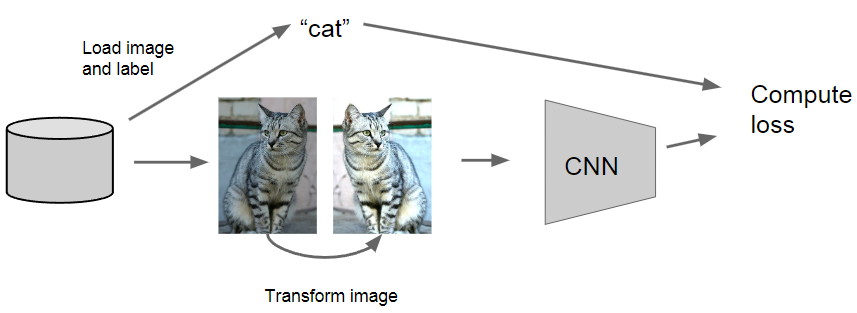
\includegraphics[width=0.42\textwidth]{pic/Lec7/Data Augmentation}
    \caption{Data Augmentation}
\end{figure}

数据扩增. 例如:
\begin{enumerate}
    \item 水平翻转
    \item 随机裁剪与缩放
    \item 颜色抖动, 随机对比度与亮度. 
\end{enumerate}

\subsection{Transfer Learning}

\begin{figure}[!htb]
    \centering
    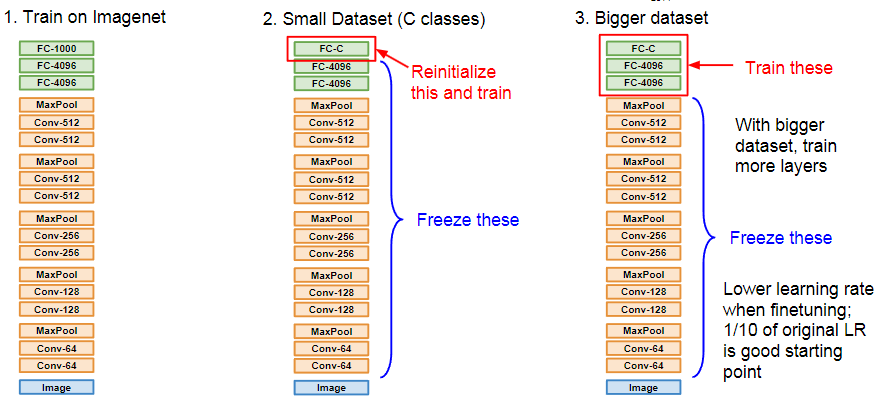
\includegraphics[width=0.42\textwidth]{pic/Lec7/Transfer Learning with CNNs}
    \caption{Transfer Learning with CNNs}
\end{figure}

只训练一部分模型以适应新的任务. 
